\chapter{Firewall}

The goals of this assignment include:
\begin{itemize}
\item Familiarizing ourselves with firewalls.
\item Correctly configuring the different options.
\item Configuring a local area network, establishing different security polices using filtering and traffic monitoring.
\item Solve a case study about connecting an SME network to the Internet using a firewall.
\end{itemize}

\section{Home preparation}
Read
\url{www.jaumebarcelo.info/teaching/lxs/ipsec/ASA_Getting_Started.pdf}
and all the assignment, and prepare a solution for the ``case study''.

\section{Configuring the working place}
Each group needs 3 PCs and a Cisco ASA 5505 firewall.

One of the PCs will be connected to the patch panel.
Before disconnecting this PC from the Internet, download an FTP server (e.g. Filezilla)
The other two, are connected to the two internal ports of the firewall.

The firewall and the external PC will be connected to the patch panel and switch B.
The external IP of the firewall will be configured according to the figure (where X is the group number).
Configure the default gateway of the PCs with the corresponding firewall interface (internal for the internal PCs and external for the external PCs).

\begin{figure}
\centering
\ifpdf
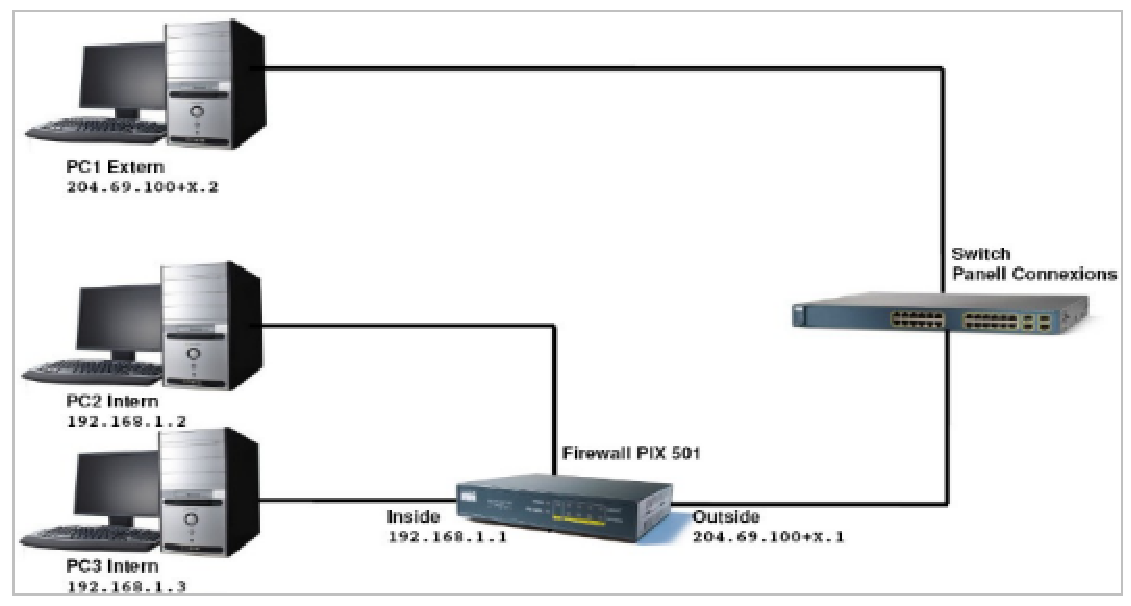
\includegraphics[width=0.9\linewidth]{Figures/firewall_topology.pdf}
\else
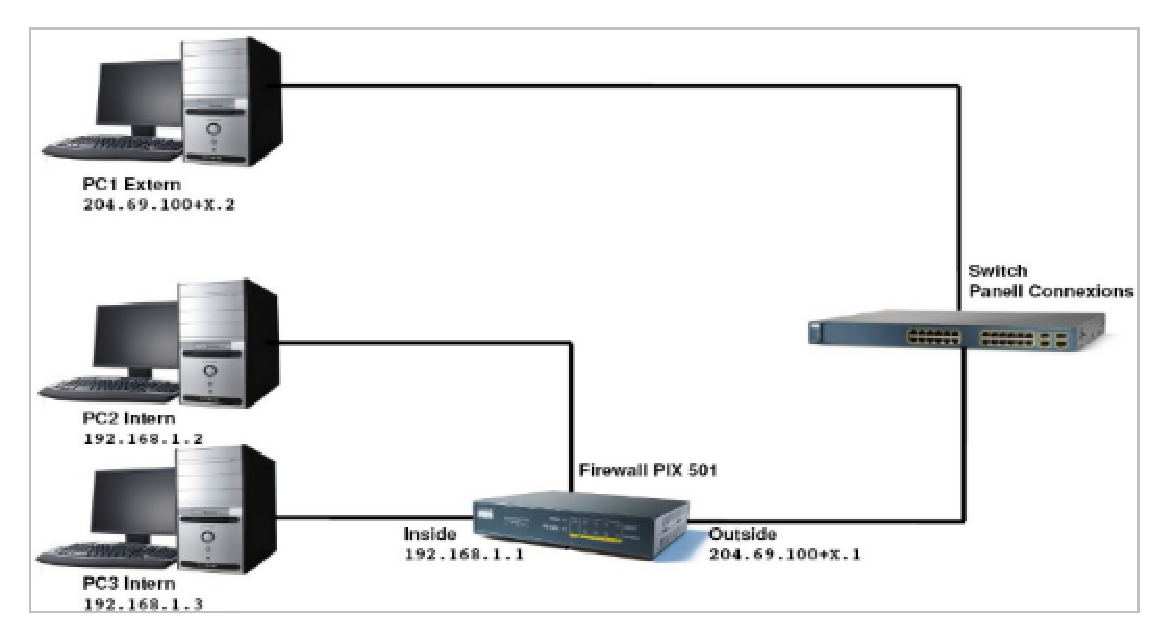
\includegraphics[width=0.9\linewidth]{Figures/firewall_topology.eps}
\fi
\caption{Network topology of the firewalls lab assignment}
\label{fig:firewall_topology}
\end{figure}

We will use FTP to verify that configuration works.
Identify the layer-4 protocol and the port number of FTP.

\section{Adaptive Security Device Manager (ASDM)}

The firewall can be configured using a Java tool which is called Adaptive Security Device Manager (ASDM).
This tool makes it possible to interact with the firewall using a web interface.
Use a windows box to run ASMD.

We will find the ``ASMD launcher'' on the desktop.
The default username and password is blank/blank.
The default IP address is 192.168.1.1 .

The CISCO ASA firewalls assign a ``security level'' to the interfaces.
A security level of 100 means the interface is 100\% trusted.
A security level of 0 means that the interface is not trusted at all.
We will check the interfaces available and their security level.
Discuss the appropriateness of this configuration.

We try to ping between the two PCs connected to the internal interfaces.

\begin{center}
\sffamily\small
\begin{tabular}{>{\columncolor{tablegray}}p{15cm}}
\rowcolor{tableheader}
\multicolumn{1}{>{\columncolor{tableorange}}l}{Question}\\
Does it work? Why?\\
\hline
\end{tabular}
\end{center}

\section{Default configuration of the ASA 5505}
The Cisco ASA use the same OS that the other devices used in the previous assignments, the Cisco IOS.
We will click on options$\rightarrow$preferences and activate ``preview commands before sending them to the device''.
This will show us the equivalent commands that would be used on the console to change the configuration.

Explain which is the default configuration of the firewall.
Observe and explain the different aspects that can be configured using the icons on the left hand side of the screen.

\begin{center}
\sffamily\small
\begin{tabular}{>{\columncolor{tablegray}}p{15cm}}
\rowcolor{tableheader}
\multicolumn{1}{>{\columncolor{tableorange}}l}{Question}\\
What is the default configuration of Ethernet 0/0 (outside)?\\
\hline
Why do you thing that the router ships with this configuration?\\
\hline
\end{tabular}
\end{center}

We will change the address of the Ethernet 0/0 (outside) interface to 204.69.100+X.1. 
Remember that the X is the group number.
We will use a /24 network mask.
Now we connect the outside PC (via switch B) to the outside interface.
We configure the IP of the outside PC to an address of the outside rang and we set the firewall's outside address as the PC's default gateway.

\begin{center}
\sffamily\small
\begin{tabular}{>{\columncolor{tablegray}}p{15cm}}
\rowcolor{tableheader}
\multicolumn{1}{>{\columncolor{tableorange}}l}{Question}\\
Can you ping from the outside PC to an inside PC? Why?\\
\hline
Whats the difference compared to the previous case?\\
\hline
\end{tabular}
\end{center}
Look at the syslog (home screen) to answer this questions.

\section{Firewall}
An alternative configuration option is telnet.
Enable the telnet option 
